%\section{ТЗ:}



\begin{lstlisting}[label=some-code,caption=Программа 1.]
#include <stdio.h>
#include <unistd.h>
#include <stdlib.h>

#define OK 0
#define ERROR 1
#define SLEEP_TIME 2
#define ERROR_FORK -1

int main()
{
	int childpid_1, childpid_2;

	// Первый процесс.
	// Создается дочерний процесс
	if ((childpid_1 = fork()) == ERROR_FORK)
	{
		// Если при порождении процесса произошла ошибка.
		perror("Can\'t fork.\n");
		return ERROR;
	}
	else if (!childpid_1)
	{
		// Это процесс потомок.
		printf("First child: id: %d ppid: %d  pgrp: %d\n", getpid(), getppid(), getpgrp());
		sleep(SLEEP_TIME);
		exit(OK);
	}

	// Аналогично 2 процесс.
	if ((childpid_2 = fork()) == ERROR_FORK)
	{
		perror("Can\'t fork.\n");
		return ERROR;
	}
	else if (!childpid_2)
	{
		// Это процесс потомок.
		printf("Second child: id: %d ppid: %d  pgrp: %d\n", getpid(), getppid(), getpgrp());
		sleep(SLEEP_TIME);
		exit(OK);
	}

	printf("Parent: id: %d pgrp: %d child1: %d child2: %d\n", getpid(), getpgrp(), childpid_1, childpid_2);

	return OK;
}
\end{lstlisting}

\begin{figure}[ht!]
	\centering{
		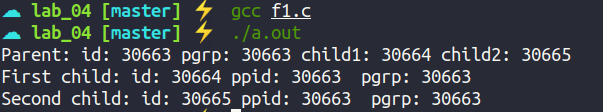
\includegraphics[width=0.8\textwidth]{img/1.png}
		\caption{Результат работы программы 1.} }
\end{figure}

\begin{lstlisting}[label=some-code,caption=Программа 2.]
#include <stdio.h>
#include <unistd.h>
#include <sys/wait.h>
#include <stdlib.h>

#define OK 0
#define ERROR 1
#define ERROR_FORK -1
#define SLEEP_TIME 2

void check_status(int status);

int main()
{
	int childpid_1, childpid_2;

	if ((childpid_1 = fork()) == ERROR_FORK)
	{
		// Если при порождении процесса произошла ошибка.
		perror("Can\'t fork.\n");
		return ERROR;
	}
	else if (!childpid_1)
	{
		// Это процесс потомок.
		printf("First child: id: %d ppid: %d  pgrp: %d\n", getpid(), getppid(), getpgrp());
		sleep(SLEEP_TIME);
		exit(OK);
	}

	// Аналогично 2 процесс.
	if ((childpid_2 = fork()) == ERROR_FORK)
	{
		perror("Can\'t fork.\n");
		return ERROR;
	}
	else if (!childpid_2)
	{
		// Это процесс потомок.
		printf("Second child: id: %d ppid: %d  pgrp: %d\n", getpid(), getppid(), getpgrp());
		sleep(SLEEP_TIME);
		exit(OK);
	}

	int status;
	pid_t child_pid;

	child_pid = wait(&status);
	printf("status: %d, child_pid: %d\n", status, child_pid);
	check_status(status);

	child_pid = wait(&status);
	printf("status: %d, child_pid: %d\n", status, child_pid);
	check_status(status);

	printf("Parent: id: %d pgrp: %d child1: %d child2: %d\n", getpid(), getpgrp(), childpid_1, childpid_2);

	return OK;
}

void check_status(int status)
{
	if (WIFEXITED(status))
	{
		printf("Дочерний процесс завершен нормально.\n\n");
		return;
	}

	if (WEXITSTATUS(status))
	{
		printf("Код завершения дочернего процесса %d.\n", WIFEXITED(status));
		return;
	}

	if (WIFSIGNALED(status))
	{
		printf("Дочерний процесс завершается неперехватываемым сигналом.\n");
		printf("Номер сигнала %d.\n", WTERMSIG(status));
		return;
	}

	if (WIFSTOPPED(status))
	{
		printf("Дочерний процесс остановился.\n");
		printf("Номер сигнала %d.", WSTOPSIG(status));
	}
}
\end{lstlisting}


\begin{figure}[ht!]
	\centering{
		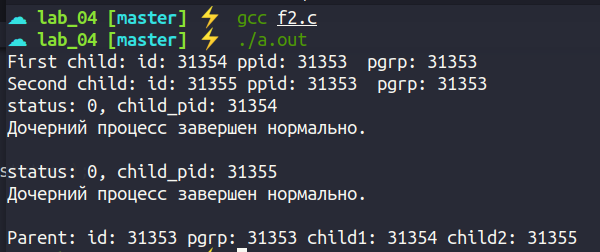
\includegraphics[width=0.8\textwidth]{img/2.png}
		\caption{Результат работы программы 2.} }
\end{figure}


